\documentclass[
  11pt,
  letterpaper,
  % addpoints,
  answers
]{exam}

\usepackage{../tarea}

\begin{document}
\begin{minipage}{0.42\textwidth}
    
\includegraphics[width=\textwidth]{../fcfm_die}
\end{minipage}
\begin{minipage}{0.53\textwidth}
\begin{center} 
\large\textbf{} \\
\normalsize Prof.~Gonzalo Narváez.
\end{center}
\end{minipage}

\vspace{0.5cm}
\noindent
\begin{questions}



\question Resuelva el siguiente problema utilizando la carta Smith. Se tiene una línea de transmisión vista en la \cref{fig:lt}, de impedancia característica $Z_c = \qty{80}{\ohm}$ y una carga $Z_l = \complexqty{70+40j}{\ohm}$.
    
    \begin{center}
      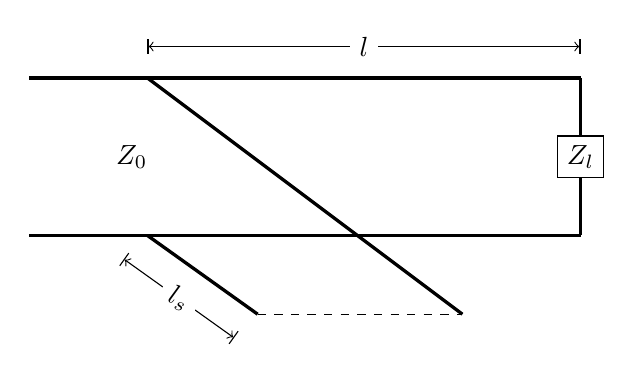
\begin{tikzpicture}
        % Línea de transmisión
        \draw[very thick] (-4,1) -- (3,1); 
        \draw[very thick] (-4,-1) -- (3,-1);
  
  
        %stub
        \draw[very thick] (-2.5,1) -- (1.5,-2);
        \draw[very thick] (-2.5,-1) -- (-1.1,-2);
  
        \draw[|<->|] (-2.5,1.4) -- (3,1.4) node[midway, fill=white] {$l$};
  
        \draw[|<->|] (-2.5-.3,-1-.3) -- (-1.1-.3,-2-.3) node[midway, rotate=-22, fill=white] {$l_s$};
        \draw[dashed] (-1.1,-2) -- (1.5,-2);
          
        %impedanciia Z_l
        \node[draw] (ZL) at (3,0) {$Z_l$};
        \draw[very thick] (3,1) -- (ZL.north);
        \draw[very thick] (3,-1) -- (ZL.south);

        
        \node at (-2.7,0) {$Z_0$};
      
    
      \end{tikzpicture}
      \captionof{figure}{Línea de transmisión original con un \textit{stub} adaptado.}
      \label{fig:lt}
    \end{center}

    Para adaptar la línea determine:
    \begin{parts}
      \part[3]{La distancia $l$ con tal de adaptar la parte real de la admitancia.}
  
      \part[4]{La distancia $l_s$ con tal de adaptar la parte imaginaria de la línea de transmisión tanto en corto circuito ($l_\text{s}^\text{cc}$) como en circuito abierto ($l_\text{s}^\text{ca}$).}
  
      \part[3]{Explique el proceso de adaptación.}
    \end{parts}
    
    \begin{solution}
      \begin{parts}
        \part{Dado que la impedancia viene dada por $Z_{l} = \complexqty{70 +j40}{\ohm}$, luego la impedancia normalizada es $z_{l}= \complexnum{0.875 +0.5j}$, mientras que su admitancia normalizada vendrá dada por $y_{l} =\complexnum{0.86-0.5j}$, extendiendo los valores de $y_{l}$ a los extremos de la carta smith se obtiene un valor aproximado de $0.375\lambda$, una vez formada la circunferencia unitaria se extiende la línea en la intersección obteniendo $\num{0.145}\lambda$, con lo que finalmente se obtiene una admitancia de la forma $y_{l}= \complexnum{1 + 0.55j}$.Para adaptar la línea nos deberemos desplazar una distancia $l = \num{0.17} \lambda $ en dirección al generador, con lo que adaptamos su parte real.}

        \part{Para obtener la distancia a la que el \textit{stub} adaptará la parte compleja $\complexnum{1.4j}$, se realiza la extension hacia el $\complexnum{-1.4j}$ para eliminar la parte compleja, y se desplaza en dirección hacia la carga hasta el extremo derecho de la carta Smith, dando un valor de $l_\text{cc}= \num{0.17}\lambda$ para el caso de circuito cerrado, mientras que para el circuito abierto se obtiene $l_\text{ca} = \num{0.42} \lambda$}.
        
        \part{El alumno debe describir el uso de la admitancia y la razón de la intersección con la circunferencia unitaria para la adaptación de la parte real, además debe comentar porque se elimina la parte compleja y como se realiza dicho proceso.}
      \end{parts}
    \end{solution} 



\end{questions}
\end{document}
